\documentclass[border=6pt]{standalone}
\usepackage{tikz}
\usetikzlibrary{positioning,arrows.meta,calc,fit}
\begin{document}
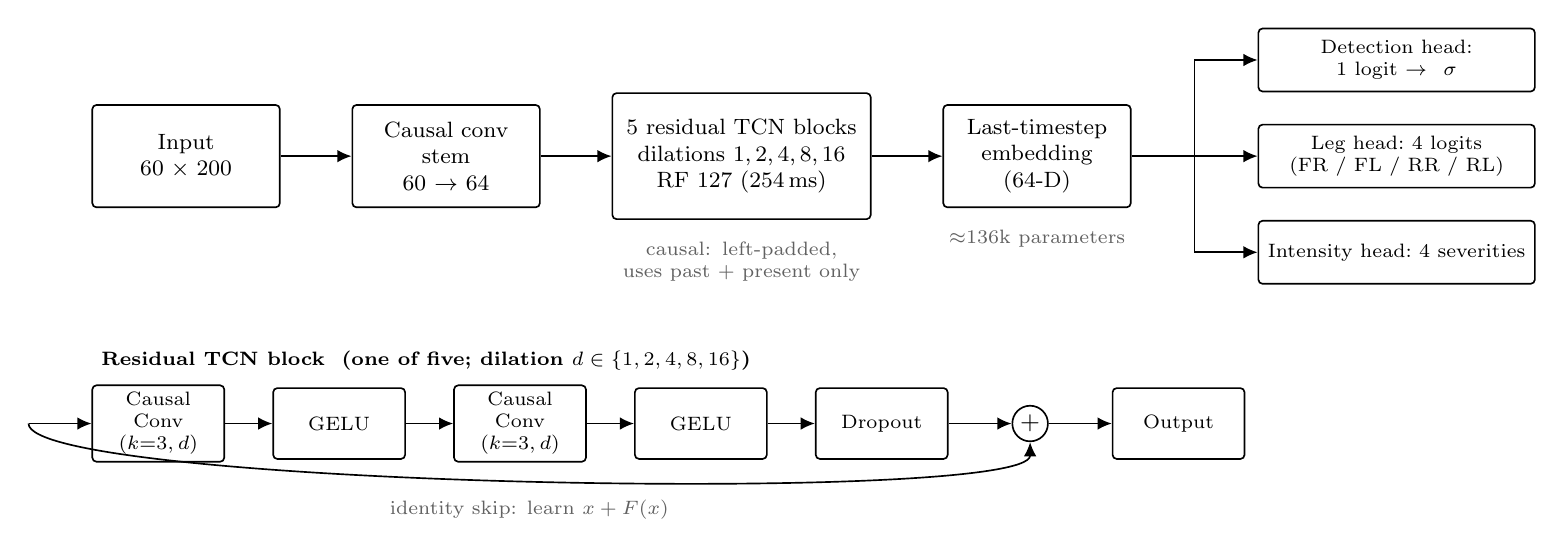
\begin{tikzpicture}[
  font=\footnotesize,
  box/.style={draw,semithick,rounded corners=1.5pt,align=center,inner sep=4pt,
              minimum height=13mm,text width=21mm,fill=white},
  wide/.style={box,text width=30mm,minimum height=16mm},
  head/.style={draw,semithick,rounded corners=1.5pt,align=center,font=\scriptsize,
               inner sep=3pt,minimum height=8mm,text width=33mm,fill=white},
  ibox/.style={draw,semithick,rounded corners=1.5pt,align=center,font=\scriptsize,
               inner sep=2.5pt,minimum height=9mm,text width=15mm,fill=white},
  op/.style={draw,semithick,circle,inner sep=1.2pt,font=\small,fill=white},
  flow/.style={-{Latex[length=1.8mm,width=1.6mm]},semithick},
  note/.style={font=\scriptsize,text=black!62}
]

% ---- main chain ----
\node[box] (in) {Input\\$60\times200$};
\node[box,right=9mm of in] (stem) {Causal conv\\stem\\$60\!\to\!64$};
\node[wide,right=9mm of stem] (blk) {5 residual TCN blocks\\dilations $1,2,4,8,16$\\RF $127$ (254\,ms)};
\node[box,right=9mm of blk] (emb) {Last-timestep\\embedding\\(64-D)};

\node[head,right=16mm of emb] (leg) {Leg head:\ 4 logits\\(FR / FL / RR / RL)};
\node[head,above=4mm of leg] (det) {Detection head:\ 1 logit $\to\sigma$};
\node[head,below=4mm of leg] (int) {Intensity head:\ 4 severities};

\draw[flow] (in)--(stem);
\draw[flow] (stem)--(blk);
\draw[flow] (blk)--(emb);
\coordinate (fan) at ($(emb.east)+(8mm,0)$);
\draw[semithick] (emb.east)--(fan);
\draw[flow] (fan) |- (det.west);
\draw[flow] (fan) -- (leg.west);
\draw[flow] (fan) |- (int.west);

\node[note,below=1.5mm of blk,text width=34mm,align=center]
     {causal: left-padded, uses past $+$ present only};
\node[note,below=1.5mm of emb] {$\approx$136k parameters};

% ---- residual-block inset ----
\node[font=\scriptsize\bfseries,anchor=west] at ($(in.west)+(0,-26mm)$) (title)
     {Residual TCN block \ (one of five; dilation $d\in\{1,2,4,8,16\}$)};
\node[ibox,below=3mm of title.west,anchor=north west] (c1) {Causal\\Conv $(k{=}3,d)$};
\node[ibox,right=6mm of c1] (g1) {GELU};
\node[ibox,right=6mm of g1] (c2) {Causal\\Conv $(k{=}3,d)$};
\node[ibox,right=6mm of c2] (g2) {GELU};
\node[ibox,right=6mm of g2] (dp) {Dropout};
\node[op,right=8mm of dp] (pl) {$+$};
\node[ibox,right=8mm of pl] (out) {Output};
\coordinate (bin) at ($(c1.west)-(8mm,0)$);

\draw[flow] (bin)--(c1);
\draw[flow] (c1)--(g1);
\draw[flow] (g1)--(c2);
\draw[flow] (c2)--(g2);
\draw[flow] (g2)--(dp);
\draw[flow] (dp)--(pl);
\draw[flow] (pl)--(out);
\draw[flow] (bin) .. controls +(0,-8mm) and +(0,-8mm) .. (pl.south);
\node[note,anchor=north] at ($(bin)!0.5!(pl |- bin)+(0,-8.5mm)$) {identity skip: learn $x+F(x)$};

\end{tikzpicture}
\end{document}
